\documentclass[a4paper]{article}

\usepackage[english]{babel}
\usepackage{amsmath}
\usepackage{color}
\usepackage{amssymb}
\usepackage{dsfont}
\usepackage{multicol}
%\usepackage[lofdepth,lotdepth]{subfig}  This gives errors when used together with "subcaption", which is needed to create subfigures.
\usepackage{graphicx}
\usepackage{listings}
\usepackage[hyphens]{url}
\usepackage{pgf, tikz}
\usetikzlibrary{arrows, automata}
\usepackage{titling}
\usepackage{varwidth}
\usepackage{hyperref}
\usepackage{color} %red, green, blue, yellow, cyan, magenta, black, white
\definecolor{mygreen}{RGB}{28,172,0} % color values Red, Green, Blue
\definecolor{mylilas}{RGB}{170,55,241}
\setlength\parindent{0pt}
\usepackage{float}
\usepackage{subcaption}
\usepackage{polynom}
\usepackage{physics}
\newcommand\tab[1][1cm]{\hspace*{#1}}


\newcommand\independent{\protect\mathpalette{\protect\independenT}{\perp}}
\def\independenT#1#2{\mathrel{\rlap{$#1#2$}\mkern2mu{#1#2}}}

\usepackage{geometry}
 \geometry{
 a4paper,
 total={165mm,257mm},
 left=20mm,
 top=20mm,
 }

\definecolor{codegreen}{rgb}{0,0.6,0}
\definecolor{codegray}{rgb}{0.5,0.5,0.5}
\definecolor{codepurple}{rgb}{0.58,0,0.82}
\definecolor{backcolour}{rgb}{0.95,0.95,0.92}

\lstdefinestyle{mystyle}{
    backgroundcolor=\color{backcolour},   
    commentstyle=\color{codegreen},
    keywordstyle=\color{magenta},
    numberstyle=\tiny\color{codegray},
    stringstyle=\color{codepurple},
    basicstyle=\footnotesize,
    breakatwhitespace=false,         
    breaklines=true,                 
    captionpos=b,                    
    keepspaces=true,                 
    numbers=left,                    
    numbersep=5pt,                  
    showspaces=false,                
    showstringspaces=false,
    showtabs=false,                  
    tabsize=2
}
 
\lstset{style=mystyle}


\DeclareMathOperator*{\argmax}{arg\,max}
\DeclareMathOperator*{\argmin}{arg\,min}

\title{Statistical Machine Learning 2018\\Assignment 4\\Deadline: 11th of January 2019}
\author{
  Christoph Schmidl\\ s4226887\\      \texttt{c.schmidl@student.ru.nl}
  \and
  Mark Beijer\\ s4354834\\     \texttt{mbeijer@science.ru.nl}
}
\date{\today}

\begin{document}
\maketitle


\section*{Exercise 1 - Logistic regression (weight 5)}

\textbf{Part 1 - The IRLS algorithm}\\

Many machine learning problems require minimizing / maximizing some function $f(x)$. For this, an alternative to the familiar gradient descent technqiue, is the so called Newton-Raphson iterative method:

\begin{eqnarray} \label{eq:1}
\textbf{x}^{(n+1)} = \textbf{x}^{(n)} - \textbf{H}^{-1} \nabla f(\textbf{x}^{(n)})
\end{eqnarray}

where \textbf{H} represents the Hessian matrix of second derivatives of $f(\textbf{x})$, see Bishop, §4.3.3.

\subsection*{1.1.1}

Derive an expression for the minimization / maximization of the function $f(x) = \sin(x)$, using the Newton-Raphson iterative optimization scheme (\ref{eq:1}), and verify (using Matlab, just up to, e.g., five iterations) how quickly it converges when starting from $x^{(0)} = 1$. What happens when you start from $x^{(0)} = -1$?\\
Hint: The Hessian of a 1-dimensional function $f(x)$ is just the second derivative $f''$. So, the Newton-Raphson iterative method reduces in 1-d to 

\begin{eqnarray}  \label{eq:2}
x^{(n+1)} = x^{(n)} - \frac{f'(x^{(n)})}{f''(x^{(n)})}
\end{eqnarray}


\textbf{Answer:}\\







\subsection*{1.1.2}


We want to apply this method to the logistic regression model for classification (see Bishop, §4.3.2):

\begin{equation}  \label{eq:3}
p(\mathcal{C}_1 | \phi ) = y(\phi) = \sigma(w^T \phi)
\end{equation}

For a data set $\{ \phi_n, t_n\}^N_{n=1}$, with $t_n \in \{ 0,1 \}$, using $y_n = p(\mathcal{C}_1 | \phi_n)$ the corresponding cross entropy error function to minimize is 

\begin{equation}  \label{eq:4}
E(\textbf{w}) = - \sum^N_{n=1} \{ t_n \ln y_n + (1 - t_n) \ln(1 - y_n)\}
\end{equation}

With one basis function $\phi$ and the dummy basis function 1, the feature vector in (\ref{eq:3}) becomes $\phi = [1, \phi]^T$. The weight vector including the bias term is then also two dimensional, $\textbf{w} = [w_0,w_1]^T$.
Expressions for the gradient $\nabla E(\textbf{w})$ and Hessian \textbf{H} in terms of the data set are given in Bishop, eq.4.96-98. As both are implicitly dependent on the weights \textbf{w}, they have to be recalculated after each step: hence this is known as the 'Iterative Reweighted Least Squares' algorithm.\\

Consider the following data set: $\{ \phi_1, t_1 \} = \{0.3, 1 \}, \{ \phi_2, t_2 \} = \{ 0.44, 0 \}, \{ \phi_3, t_3 \} = \{ 0.46, 1 \}$ and $\{ \phi_4, t_4 \} = \{ 0.6, 0 \}$, and initial weight vector $\textbf{w}^{(0)} = [1.0, 1.0]^T$.\\

Show using e.g. a Matlab implementation that for this situation the IRLS algorithm converges in a few iterations to the optimal solution $\hat{\textbf{w}}^T \approx [9.8, -21.7]$, and show that this solution corresponding to a decision boundary $\phi = 0.45$ in the logistic regression model. (The IRLS algorithm should take about five lines of Matlab code inside a loop + initialization).\\


\textbf{Answer:}\\



\textbf{Part 2 - Two-class classification using logistic regression}\\

\begin{figure}[H]
\center
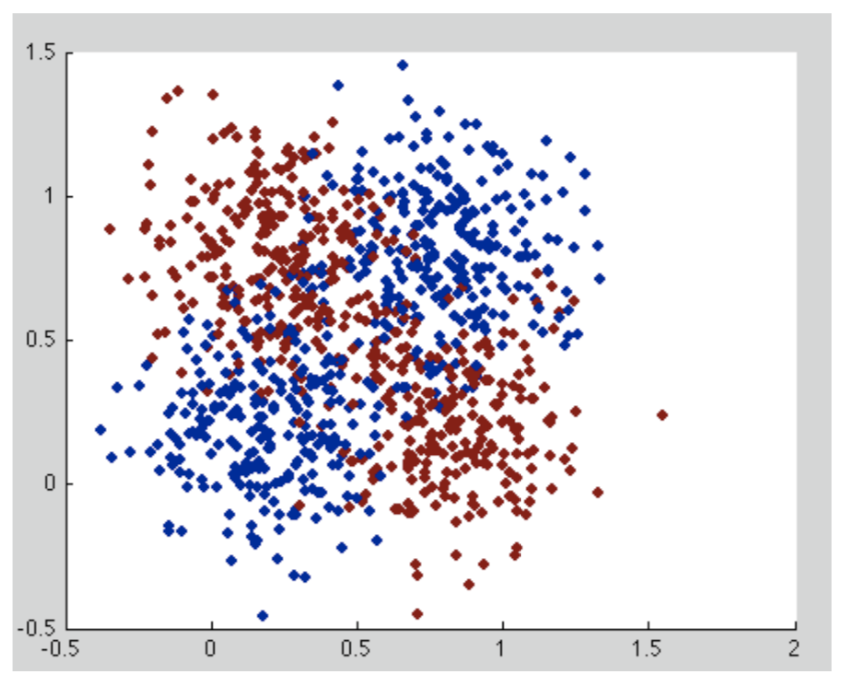
\includegraphics[width=0.4\textwidth]{Images/two-class-dataset.png}
\caption{Two class data for logistic regression}
\label{Fig:two-class-dataset}
\end{figure}

Two-class classification using logistic regression in the IRLS algorith,. Data consists of 1000 pairs $\{ x_1, x_2 \}$ with corresponding class labels $\mathcal{C}_1 = 0$ or $\mathcal{C}_2 = 1$. Load it into Matlab using\\

\hspace{1cm} \texttt{data = load('a010\_irlsdata.txt', '-ASCII');}

\hspace{1cm} \texttt{X = data(:,1:2); Y = data(:,3);}\\

\subsection*{1.2.1}

Make a scatter plot of the data, similar to Figure \ref{Fig:two-class-dataset}. (Have a look at Matlab file \texttt{a010plotideas.m} in Brightspace for some ideas to make such a scatter plot and the plots later on.) Do you think logistic regression can be a good approach to classification for this type of data? Explain why.\\

\textbf{Answer:}\\






\subsection*{1.2.2}

Modify the Iterative Reweighted Least Squares algorithm from part 1 to calculate the optimal weights for this data. Use again a dummy basis function. Initialize with the weight vector $\textbf{w}^T = [0, 0, 0]$. With these initial weights, what are the class probabilities according to the logistic regression model (i.e., before optimization)?\\

\textbf{Answer:}\\








\subsection*{1.2.3}

Run the algorithm. Make a scatter plot of the data, similar to figure \ref{Fig:two-class-dataset}, but now with color that represent the data point probabilities $P(C = 1, X_n)$ according to the model after optimization. Compare the cross entropy error with the initial value. Did it improve? Much? Explain your findings.\\

\textbf{Answer:}\\







\subsection*{1.2.4}

Introduce two Gaussian basis functions as features $\phi_1, \phi_2$, similar to Bishop, fig.4.12. Use identical isotropic covariance matrices $\Sigma = \sigma^2 I$ with $\sigma^2 = 0.2$, and center the basis functions around $\mu_1 = (0,0)$ and $\mu_2 = (1,1)$. Make a scatter plot of the data in the feature domain. Do you think logistic regression can be a good approach to classification with these features? Explain why.\\

\textbf{Answer:}\\










\subsection*{1.2.5}

Modify the IRLS algorithm to use the features $\{ \phi_1, \phi_2 \}$ and the dummy basis function. Initialize with the weight vector $\textbf{w}^T = [0,0,0]$.\\
Run the algorithm. Make a scatter plot of the data, similar to Figure \ref{Fig:two-class-dataset}, but now with colors that represent the data point probabilities $P(C = 1 | X_n)$ according to this second model (after optimization). Compare the cross entropy error with the initial value. Did it improve? Much? Explain your findings.\\


\textbf{Answer:}\\


\section*{Exercise 2 - Neural network regression (weight 5)}

We train a neural network using backpropagation, to learn to mimic a 2D multimodal probability density. First, we implement the network and test its regression capabilities on a standard Gaussian; then we train it on the real data set. Visualization of the network output plays an important role in monitoring the progress.

\subsection*{2.1}

Create a plot of an isotropic 2D Gaussian $y = 3 \cdot \mathcal{N}(\textbf{0}|\frac{2}{5}\textbf{I}_2)$ centered at the origin using the \texttt{meshgrid()}, \texttt{mvnpdf()} and \texttt{surf()} functions. Sample the density at 0.1 intervals over the range $[-2,2] \times [-2,2]$ and store the data in colum vector variables $\textbf{X}$ (2D) and $\textbf{Y}$ (1D).\\

\textbf{Answer:}\\







\subsection*{2.2}

Implement a 2-layer neural network with $D = 2$ input nodes, $K = 1$ output nodes and $M$ hidden nodes in the intermediate layer that can be trained using a sequential error backpropagation procedure, as described in Bishop §5.3. Use $tanh(\cdot)$ activation functions for the hidden nodes and a linear activation function (regression) for the output node. Introduce appropriate weights and biases, and set the learning rate parameter $\eta = 0.1$. Initialize the weights to random values in the interval $[-0.5,0.5]$. Plot a 2D graph of the initial output of the network over the same $[-2,2] \times [-2,2]$ grid as the Gaussian (again using \texttt{surf()}).\\

\textbf{Answer:}\\









\subsection*{2.3}

Train the network for $M = 8$ hidden nodes on the previously stored $\textbf{X}$ and $\textbf{Y}$ values (the $\{ x_1, x_2 \}$ input coordinates and corresponding output probability density $y$), by repeatedly looping over all datapoints and updating the weights in the network after each point. Repeat for at least 500 complete training cycles and monitor the progress of the training by plotting the output of the network over the $\textbf{X}$ grid after each full cycle. Verify the output starts to resemble the Gaussian density after some 200 cycles (all be it with lots of 'wobbles').\\


\textbf{Answer:}\\







\subsection*{2.4}

Permute the $\textbf{X}$ and $\textbf{Y}$ arrays to a random order using the \texttt{randperm()} function, keeping corresponding $x$ and $y$ together. Repeat the network training session using this randomized data set. Verify that convergence is now much quicker. Can you understand why? Try out the effect of different numbers of hidden nodes, different initial weights and different learning rates on speed and quality of the network training. Explain your results.

\begin{figure}[H]
\center
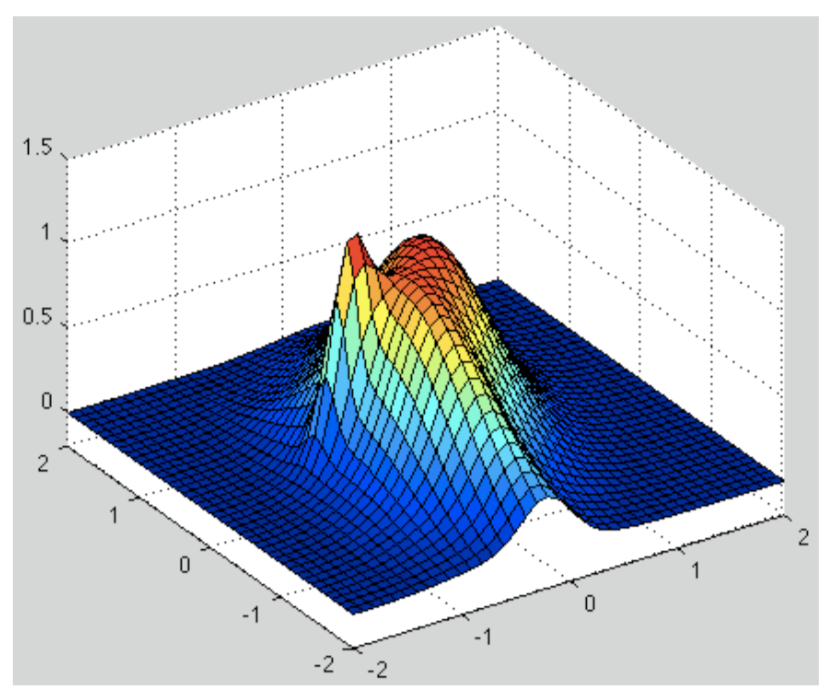
\includegraphics[width=0.4\textwidth]{Images/multi-modal.png}
\caption{Multi-modal probability density}
\label{Fig:multi-modal}
\end{figure}



After these preliminaries we are now going to train the network on the real data set.\\
Load the data using\\


\hspace{1cm} \texttt{data = load('a017\_NNpdfGaussMix.txt', '-ASCII');}

\hspace{1cm} \texttt{X = data(:,1:2); Y = data(:,3);}\\

\textbf{Answer:}\\






\subsection*{2.5}

Create a $2D$-plot of the target probability density function. Notice that the data is in the correct sequence to use in \texttt{surf()}.\\

\textbf{Answer:}\\








\subsection*{2.6}

Train the network on this data set. Use at least 40 hidden nodes and a learning rate parameter no higher than $\eta = 0.01$. Make sure the input data is properly randomized. Run the training phase for at least 2000 complete cycles and follow the progress by plotting the updated network output after every 20 full cycles. How does the final output of the network compare to the target distribution in the data? Explain. How could you improve the neural network in terms of speed of convergence and/or quality of the approximation?



\section*{Exercise 3 - Gaussian processes (weight 5)}


\textbf{Part 1 - Sampling from Gaussian stochastic processes}\\

One widely used kernel function for Gaussian process regression is given by the exponential of quadratic form, with the addition of constant and linear terms (eq. 6.63 Bishop):

\begin{eqnarray} \label{eq:5}
k(\textbf{x}, \textbf{x'}) = \theta_0 \exp(- \frac{\theta_1}{2} || \textbf{x} - \textbf{x}' ||^2) + \theta_2 + \theta_3 \textbf{x}^T \textbf{x}'
\end{eqnarray}

We denote by $\boldsymbol{\theta}  = (\theta_0, \theta_1, \theta_2, \theta_3)$ the hyperparameter vector governing the kernel function $k$.

\subsection*{3.1.1}

Implement the kernel given by Equation (\ref{eq:5}) in Matlab as a function of $\textbf{x}, \textbf{x}'$ and $\boldsymbol{\theta}$. Note that $\textbf{x}$ can have any dimension.\\

\textbf{Answer:}\\





\subsection*{3.1.2}

We first consider the univariate case. For the parameter values $\boldsymbol{\theta} = (1,1,1,1)$ and $N = 101$ equally spaced points $\textbf{X}$ in the interval $[-1,1]$, compute the Gram matrix $\textbf{K(X,X)}$ (eq. 6.54 Bishop). What is the dimension of \textbf{K}? How can we show that \textbf{K} is positive semidefinite?\\

Note: Even when \textbf{K} is positive definitive, some of its eigenvalues may be too small to accurately compute (same for the determinant). This may pose a problem when generating a multivariate Gaussian distribution using \textbf{K} as its covariance matrix. You can alleviate this issue by adding a small diagonal term to \textbf{K}.\\


\textbf{Answer:}\\







\subsection*{3.1.3}

We will now use the previously computed matrix \textbf{K(X,X)} to produce samples from the Gaussian process prior $\textbf{y(X)} ~\mathcal{N}(\textbf{0, K(X,X)})$, with \textbf{X} being the previously determined N equally spaced points. Generate five functions \textbf{y(X)} with Matlab and plot them against the N input values \textbf{X}. Repeat the process (remember to compute a new \textbf{K} each time) for the hyperparameter configurations from Bishop, Figure 6.5:

\begin{align*}
\boldsymbol{\theta} \in \{(1,4,0,0),(9,4,0,0),(1,64,0,0),(1,0.25,0,0),(1,4,10,0),(1,4,0,5)\}.
\end{align*}

Describe the differences between the plots. Explain in which way each of the kernel parameters affects the generated samples.\\


\textbf{Answer:}\\





\subsection*{3.1.4}

We now move to the bivariate case. Instead of an interval, we now consider a 2-D grid of equally spaced points of size $N = 21 \times 21$ in $[-1,1] \times [-1,1]$. We collect all these grid points in a data matrix \textbf{X}, where each one of the 441 observations has two dimensions. What is the dimension of \textbf{K} now? What does this tell you about the scalability of sampling multivariate functions from Gaussian processes in higher dimensions?\\

\textbf{Answer:}\\






\subsection*{3.1.5}

Using the same kernel from (\ref{eq:5}), compute the Gram matrix \textbf{K(X,X)} on the grid for each hyperparameter configuration $\boldsymbol{\theta} \in \{(1, 1, 1, 1), (1, 10, 1, 1), (1, 1, 1, 10)\}$. For each \textbf{K}, generate and plot four random surfaces from the Gaussian process prior $\textbf{yX()} ~\mathcal{N}\textbf{(0, K(X,X)})$. Compare the observed differences to the univariate case.\\


\textbf{Answer:}\\








\textbf{Part 2 - Gaussian processes for regression}\\



\section*{Exercise 4 - EM and doping (weight 5)}





\subsection*{3.2d}



\subsection*{3.2e}



\end{document}
